\subsection{La gestion des personnages}

Les personnages sont la pièce maîtresse de l'application. Pour la simulation il y a deux types de personnages : Pacman et les fantomes.
Ci dessous, le diagramme de classes lié aux personnages : \\[0.5cm]
\centerline{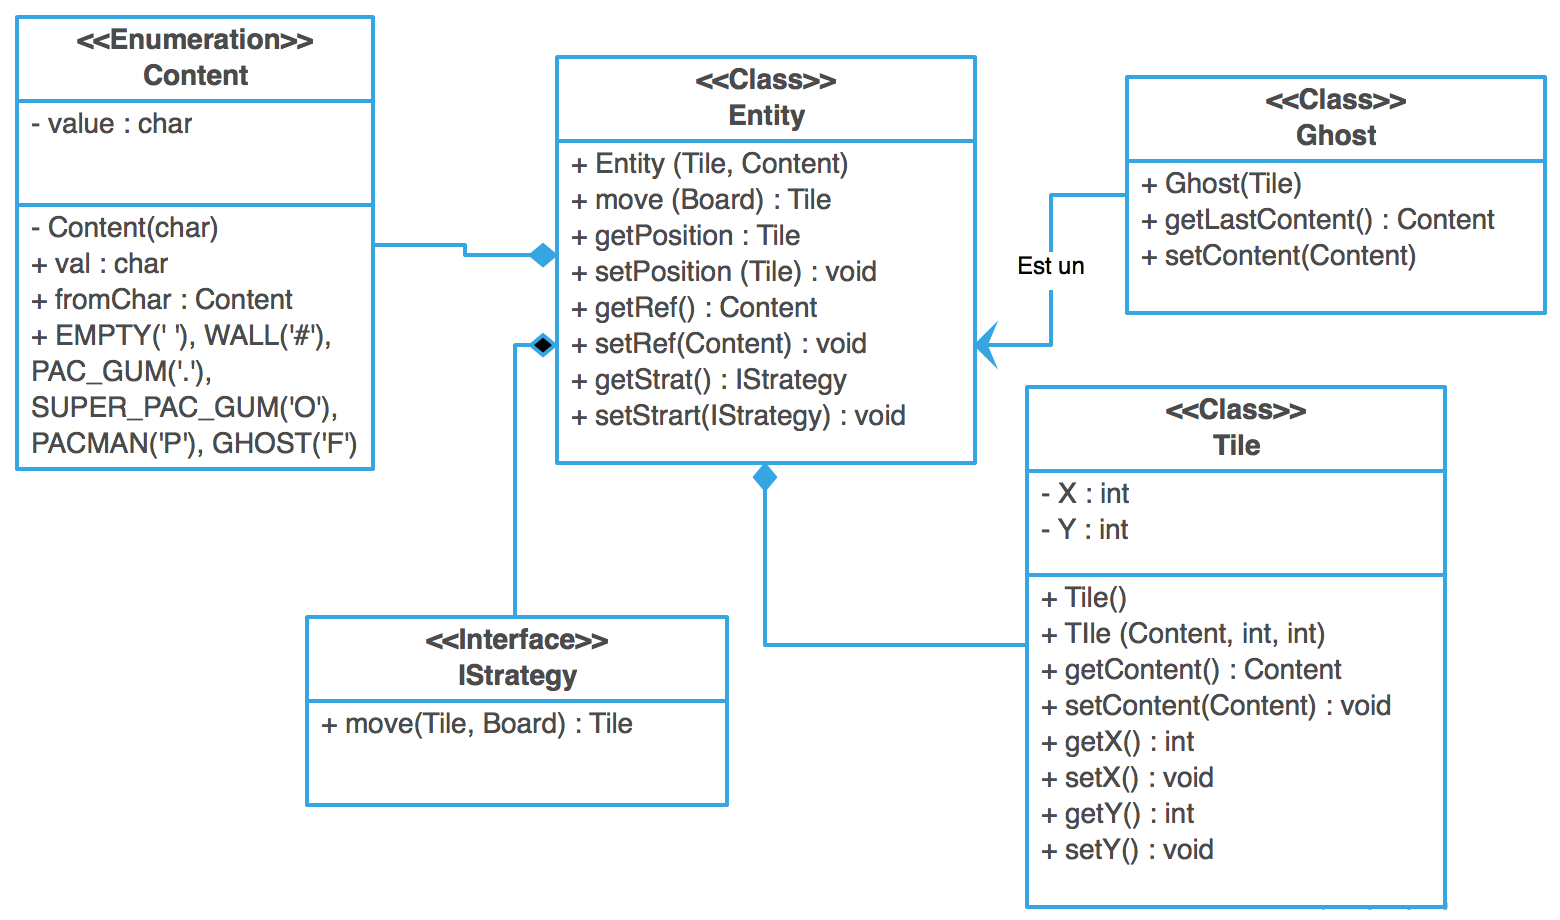
\includegraphics[scale=0.2]{Entity}}

Le premier choix était de savoir si Pacman et les fantômes seraient des classes à part entière. La seule différence notable est le fait que Pacman mange tout ce qu'il trouve sur son chemin (excepté les fantomes) tandis que les fantomes doivent se déplacer sans altérer le contenu des cases qu'ils parcourent (excepté Pacman). C'est pourquoi la classe Ghost a un attribut lastContent afin de sauvegarder le contenu (cf Enum Content dans le diagramme) de la case sur laquelle le fantome se trouve.
Ceci permettra notamment de redessiner correctement la carte après passage d'un fantome. \\
D'autre part les points communs de tous les personnages sont le fait qu'ils se deplacent. Ce déplacement nécessite donc que chaque personnage possède une position, sa position courante. La classe Tile (cf partie Gestion de la carte) sert à stocker l'emplacement de nos personages. La méthode move() du personnage retourne la nouvelle position du personnage et délègue ce calcul à la stratégie (cf partie sur les Stragtégies) du personnage.



